\chapter{Mimicking electromagnetically induced transparency in the magneto-optical activity of magnetoplasmonic nanoresonators \label{chap3}}

\section{Introduction}

In complex optical nanostructures, the electromagnetic interactions between the constituent elements strongly determine the response of the whole system. In plasmonic systems it is possible to find examples of this fact with a variety of complex architectures including core-shell particles \cite{prodan2003hybridization}, nanoantennas \cite{muhlschlegel2005resonant,fromm2004gap, ghenuche2008spectroscopic} dimers \cite{su2003interparticle, Rechberger_2003, dmitriev2007gold, wadell2012optical, brown2010heterodimers}, oligomers \cite{hentschel2010transition, lassiter2010fano}, periodic arrays \cite{zou2004silver, auguie2008collective}, etc. The control and manipulation of the interactions can give rise to strong enhancement of the electromagnetic field in subwavelength spatial regions \cite{aizpurua2005optical, sundaramurthy2005field}, the building up of bright and dark modes \cite{dolling2005cut, verellen2009fano, yang2011fano} or the Fano resonances exhibited in the optical signal \cite{luk2010fano, francescato2012plasmonic, gallinet2011influence}. These results have direct consequences in different areas and allow the development of new devices such as nanoantennas \cite{cubukcu2008plasmonic}, high sensitivity sensors \cite{cetin2012fano, anker2008biosensing} or novel telecommunication architectures/devices \cite{schuller2010plasmonics}, among others. The modification of the geometry, the spatial arrangement and the material composition of the constituting elements allow the control and even boost at will such optical responses. These morphological and configurational factors determine how the whole entity interacts with an electromagnetic field. In this scenario, the incorporation of magneto-optical character into the plasmonic system by adding a ferromagnetic component, to form the so-called magnetoplasmonic (MP) structures, introduces an additional degree of freedom. 
%Examples of the potentiality of magnetoplasmonics are the development of active plasmonic configurations whose properties can be externally tuned by the application of a magnetic field or structures with enhanced magneto-optical activity \cite{temnov2010active, belotelov2011enhanced, banthi2012high, armelles2013magnetoplasmonics, chin2013nonreciprocal}.\\
In order to study the influence of the magneto-optical (MO) activity over a plasmonic system, a very simple model is considered, where the elements of the system are described by point-like dipoles. This description is valid when the spatial field variation inside the elements is negligible, implying that these elements are considerably smaller than the wavelength. A point dipole in the presence of an external, steady, magnetic field, experiences a modification of its dipole moment that depends on the relative dipole-magnetic field orientation. In particular, if they are perpendicularly oriented, the dipole rotates due to the Lorentz force \cite{sepulveda2010plasmon}, and this rotation can be seen as a new degree of freedom for the interactions in plasmonic structures. Moreover, the Lorentz force depends on the material, being stronger for ferromagnetic components. This makes it possible to design structures where this force is spatially different by selecting different materials in its interior, therefore enriching the interaction pattern.

In this chapter we study the influence of the magneto-optical activity over a nanostructure. In Sec. (\ref{sec:chap3_coupledoscillators}) we show a mechanical equivalent to the electromagnetic (EM) problem by considering two coupled masses, where one of the mass is charged and over the system is applied a magnetic field. The results, from the phenomenological point of view, are similar to the electromagnetic case and are used to develop a more intuitive understanding of the problem. In Sec. (\ref{sec:chap3_nanoresonators}) nanodisk dimers consisting of a magnetoplasmonic and a plasmonic unit are considered, where the electromagnetic coupling is controlled via the distance between them. It is shown that, due to the electromagnetic interaction, a pronounced dip in the spectral dependence of the magneto-optical activity is observed, exhibiting a characteristic Fano shape. This reduction of the magneto-optical activity is similar to the electromagnetically induced transparency effects observed in numerous physical systems \cite{harris1990nonlinear,xu2006EIT, zhang2008plasmon, papasimakis2008metamaterial, liu2009plasmonic}.
In Sec. (\ref{sec:chap3_discussion}) and (\ref{sec:chap3_conclusions})  are presented the discussion and conclusions respectively.
%allows a clearer understanding of the electromagnetic problem.

\section{Coupled oscillators: mechanical and dipolar models\label{sec:chap3_coupledoscillators}}

Let us consider a simplified model system that assumes the plasmonic components, from a classical point of view, as masses coupled by springs (coupled spring resonators). This model has been already employed to give a simple picture for systems with two interacting plasmonic modes \cite{wadell2012optical, lassiter2010fano, joe2006classical, antosiewicz2012absorption}. It is possible to introduce in this mechanical model effects like those of a MO activity in the materials by considering charged masses in a static magnetic field. The presence of the magnetic field and a charged element give rise to the appearance of a Lorentz force $\mathbf{F}_{l} = q \dot{\mathbf{r}}\times\mathbf{B}$. In the case considered here, the static magnetic field is applied perpendicularly to the driving, external force, therefore the Lorentz force will be perpendicular to both an thus define a plane of movement. Let us say that the external force is in the $x-$direction and the magnetic field in the $z-$direction, then the Lorentz force will be in the $y-$direction, (see Fig. (\ref{fig:scheme_springsdipoles})(a), right side) and the plane of movement of the masses will be the $x-y$ plane.\\
\begin{figure}[h] %h!
\begin{centering}
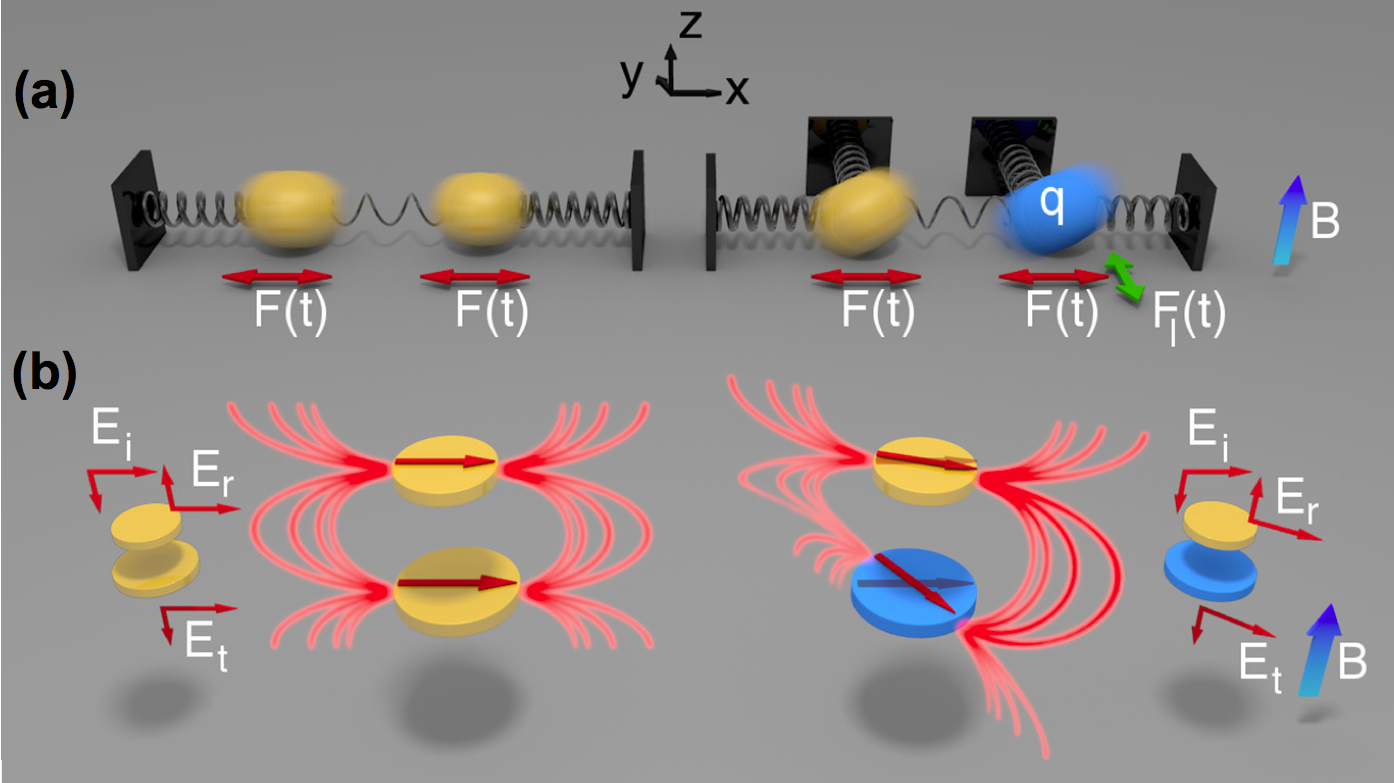
\includegraphics[width=12cm]{chapter_3/schemes/Fig_1.png} 
\par\end{centering}
\caption{ (a) Spring model representing a two coupled masses system excited by an harmonic force, $F\left(t\right)$, along $x$ axis. Left side: uncharged masses. Right side: one of the masses (blue) is charged $\left(q\right)$ and a static magnetic field $\left(\mathbf{B}\right)$ is applied along the $z-$direction, inducing a Lorentz force, $F_{1}\left(t\right)$, along the $y-$direction. The $y-$movement is transferred to the other mass through the coupling.\\
(b) Two interacting electric dipoles, representing two metallic disks, excited by an incident beam polarised along the $x$ axis. Left side: No disk has magneto-optical activity and the reflected $\left(E_{r}\right)$ and transmitted  $\left(E_{t}\right)$ light have the same polarisation direction than the incident  $\left(E_{i}\right)$ light. Right side: one of the disks (blue) has magneto-optical activity and a static magnetic field  $\left(\mathbf{B}\right)$ applied along the $z-$direction induces a rotation of its electric dipole, which is transferred to the other dipole through the interaction. The rotation modifies the polarisation direction of the reflected  $\left(E_{r}\right)$ and transmitted  $\left(E_{t}\right)$ light.\label{fig:scheme_springsdipoles}}
\end{figure}
The equations of motion are defined by:

\begin{eqnarray}
m_{1}\ddot{\mathbf{r}}_{1} & = & \mathbf{F}_{1}-k_{1}\mathbf{r}_{1}-k_{12}\left(\mathbf{r}_{1}-\mathbf{r}_{2}\right)-\mathbb{B}_{1}\dot{\mathbf{r}}_{1}, \nonumber \\
m_{2}\ddot{\mathbf{r}}_{2} & = & \mathbf{F}_{2}-k_{2}\mathbf{r}_{2}-k_{12}\left(\mathbf{r}_{2}-\mathbf{r}_{1}\right)-\mathbb{B}_{2}\dot{\mathbf{r}}_{2},
\end{eqnarray}
where the particle positions $\mathbf{r}_{i}$ are restricted to the $x-y$ plane and referred to its equilibrium
state, $k_{i}$ are spring constants, $k_{12}$ is the interaction between the particles, $m_{i}$ are their masses and, more importantly, the damping terms $\mathbb{B}_{i}$ are tensors:

\begin{eqnarray}
\mathbb{B}_{i} & = & b_{i}+F_{l}^{i}\\
 & = & \left[\begin{array}{cc}
b_{i} & 0\\
0 & b_{i}
\end{array}\right]+\left[\begin{array}{cc}
0 & -qB_{i}\\
qB_{i} & 0
\end{array}\right],
\end{eqnarray}
arising from the Lorentz force:

\begin{equation}
\mathbf{F}_{l}^{i} = qB_{i}\left[\begin{array}{cc}
0 & 1\\
-1 & 0
\end{array}\right]\left(\begin{array}{c}
\dot{r}_{x}\\
\dot{r}_{y}
\end{array}\right).
\end{equation}
It is easy to see that in the absence of a magnetic field, and considering only the friction force in a homogeneous medium, $\mathbb{B}$ can be regarded as a scalar term (diagonal with equal eigenvalues) $b$. In this case, the simple plasmonic structure without external magnetic field would be two point masses coupled in one dimension (Fig. (\ref{fig:scheme_springsdipoles})(a), left side). This system is characterised by two resonant eigenmodes, symmetric and anti-symmetric in character.\\
Is considered, without losing generality, that $m_{1} = m_{2} = m$ and that the external driving force has a harmonic temporal dependence $e^{-i\omega t}$. Thus, using the following definition:
\begin{eqnarray}
\omega_{i}^2 & = & {k_{i}}/{m} \nonumber \\
\omega_{12}^2 & = & {k_{12}}/{m}\nonumber \\
\Gamma_{i} & \equiv & \frac{\mathbb{B}_{i}}{m}\equiv \left(\begin{array}{cc}
\gamma_i & -\omega_{c,i}\\
\omega_{c,i} & \gamma_{i}
\end{array}\right),
\end{eqnarray}
the equations of motion in the frequency space become:

\begin{eqnarray}
-\mathcal{F}_{1} = \left(\omega^2 - \omega_{1}^{2} + i\omega\Gamma_{1} - \omega_{12}^{2}\right)\bold{r}_{1}+\left(\omega_{12}^2\right)\mathbf{r}_{2}\\
-\mathcal{F}_{2} = \left(\omega^2 - \omega_{2}^{2} + i\omega\Gamma_{2} - \omega_{12}^{2}\right)\bold{r}_{2}+\left(\omega_{12}^2\right)\mathbf{r}_{1},
\end{eqnarray}
where $\mathcal{F}_{i}$ is the corresponding Fourier component of the external force, $F_{i}/m\equiv\mathcal{F}_{i}$.\\
In the matrix form, this reads as:

\begin{eqnarray}
\mathbf{M}\left(\begin{array}{c}
\mathbf{r}_{1}\\
\mathbf{r}_{2}
\end{array}\right) & \equiv & \left[\begin{array}{cc}
\left(\left(\Omega_{1}^{2}-\omega_{12}^{2}\right)\mathbb{\mathbb{I}}+\omega\omega_{c,1}\sigma_{2}\right) & \omega_{12}^{2}\mathbb{I}\\
\omega_{12}^{2}\mathbb{I} & \left(\left(\Omega_{2}^{2}-\omega_{12}^{2}\right)\mathbb{\mathbb{I}}+\omega\omega_{c,2}\sigma_{2}\right)
\end{array}\right]\left(\begin{array}{c}
\mathbf{r}_{1}\\
\mathbf{r}_{2}
\end{array}\right)\nonumber \\
 & = & \left(\begin{array}{c}
-\mathcal{F}_{1}\\
-\mathcal{F}_{2}
\end{array}\right),\label{eq:chap3_mecsystem}
\end{eqnarray}
where $\mathbb{I}$ is a $2\times2$ unit matrix, $\sigma_{2}$ is the $2\times2$ Pauli matrix $\left(\sigma_{2}\equiv \left(\begin{array}{cc}
0 & -i\\
i & 0
\end{array}\right)\right)$ and $\Omega_{i}^2\equiv \omega^2 -\omega_{i}^2 + i\omega \gamma_{i}$.\\
In the problem addressed here, only one of the particles has MO activity, which is the same as to say that either $\omega_{c,1}$ or $\omega_{c,2}$ is zero (we have chosen $\omega_{c,1}$ to be zero). In order to
mimic the photonic case, the external driving force is also special, and is applied to both particles along the $x-$direction only. The solution is then:

\begin{equation}
\begin{cases}
x_1 & = - \frac{\mathcal{F}_{x}}{\cal{D}} \left[\left[\Omega_{1}^2\Omega_{2}^2-\omega_{12}^2\left(\Omega_{1}^{2}+\Omega_{2}^2\right)\right]\left(\Omega_{2}^2-2\omega_{12}^2\right)-\omega^{2}\omega_{c}^2\left(\Omega_{1}^2-\omega_{12}^2\right)\right]
\\
y_{1} & = - \frac{\mathcal{F}_{x}}{\cal{D}}\left[i\omega \omega_{c} \omega_{12}^2\left(\Omega_{1}^2-2\omega_{12}^2\right)\right] \\
x_2 & = - \frac{\mathcal{F}_{x}}{\cal{D}} \left[\left[\Omega_{1}^2\Omega_{2}^2-\omega_{12}^2\left(\Omega_{1}^{2}+\Omega_{2}^2\right)\right]\left(\Omega_{1}^2-2\omega_{12}^2\right)\right]\\
y_{2} & = - \frac{\mathcal{F}_{x}}{\cal{D}}\left[-i\omega \omega_{c} \left(\Omega_{1}^2-\omega_{12}^2\right)\left(\Omega_{1}^2-2\omega_{12}^2\right)\right],
\end{cases}\label{eq:chap3_amplitudes}
\end{equation}
where ${\cal{D}} = \omega_{12}^8 - 2\left(\Omega_{1}^2-\omega_{12}^2\right)\omega_{12}^4\left(\Omega_{2}^2-\omega_{12}^2\right) + \left[\left(\Omega_{2}^2-\omega_{12}^2\right)^2-\omega^{2}\omega_{c}^2\right]\left(\Omega_{1}^2-\omega_{12}^2\right)^2$. Details of the calculation are presented in Appendix (\ref{app:coupled_masses}).\\
In Fig. (\ref{fig:mechanicalresult}) we show the results obtained from Eq. (\ref{eq:chap3_amplitudes}), using $\mathcal{F}_x = 1 m/s^2$, $\omega_{1} = 0.9\omega_{2}$, $\gamma_{1} = 0.02\omega_2$, $\gamma_2 = 0.05\omega_{2}$, $\omega_{12} = 0.25\omega_2$, $\omega_c = 0.01\omega_{2}$.\\
Although the force is only applied in the $x-$direction and only one of the masses is charged, due to the coupling between  masses, both exhibit movement in the $y-$direction, \textit{i.e.}, from the excitation in the $x-$direction, part of the energy is converted into movement in the $y-$direction.

\begin{figure}[h!]
\begin{centering}
\par\end{centering}
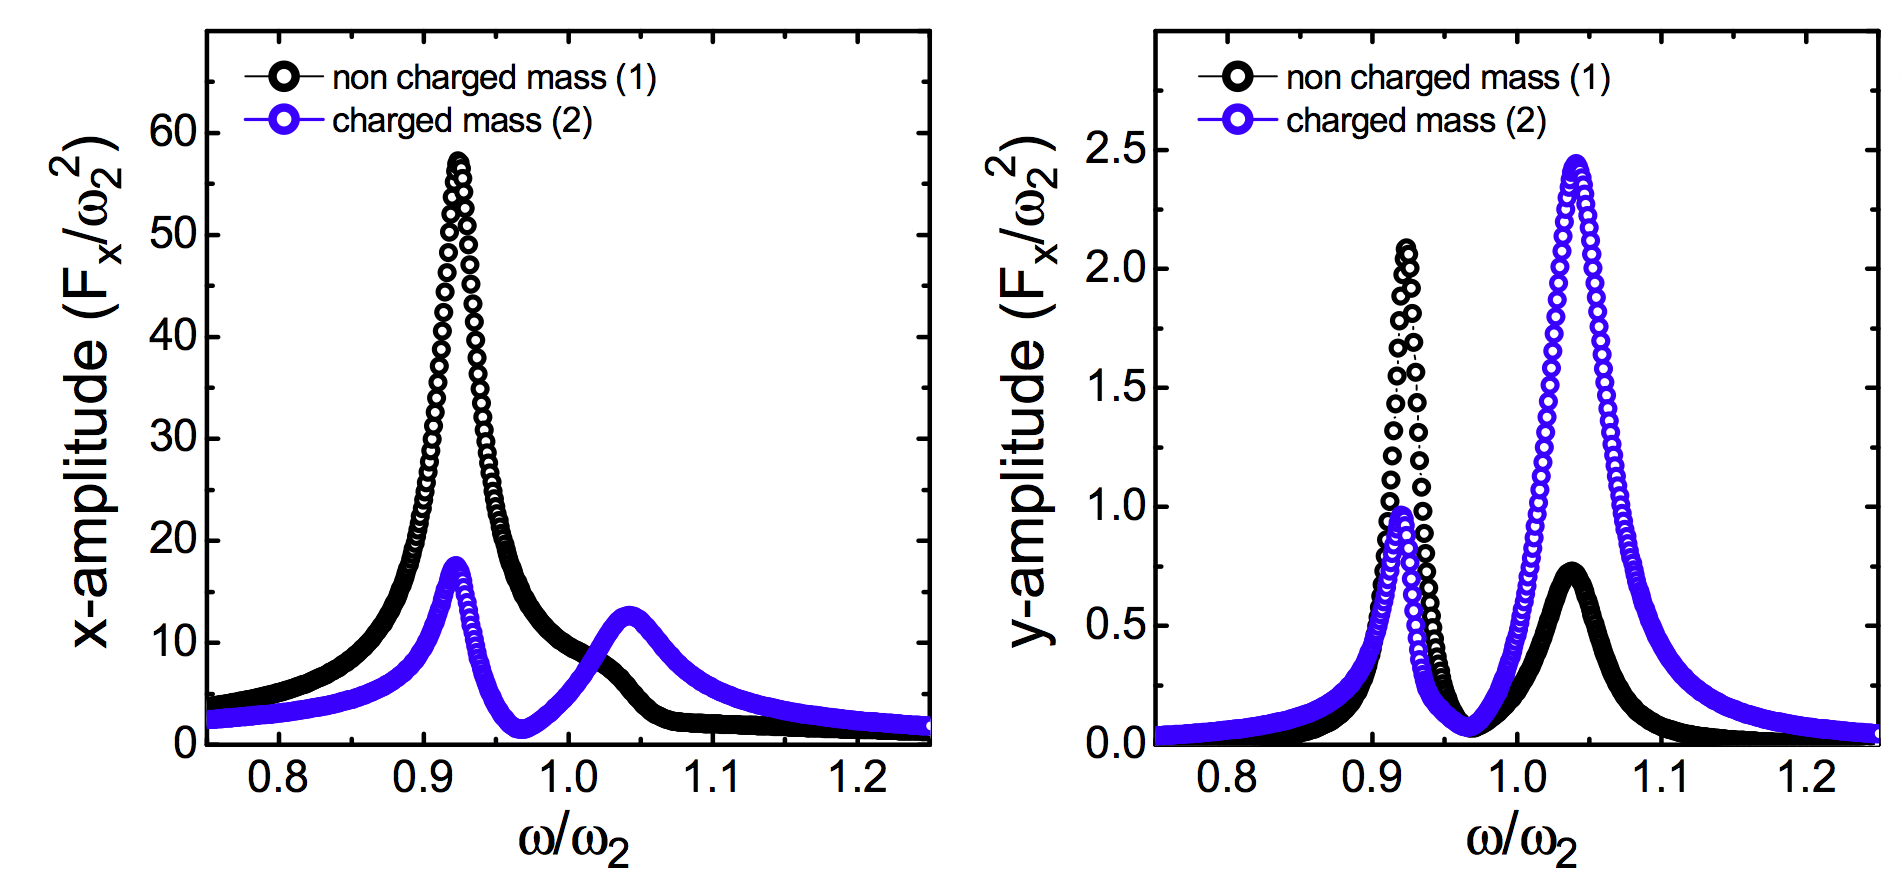
\includegraphics[width=12cm]{chapter_3/graphics/Fig_6.png} 
\caption{Oscillation amplitude as a function of the frequency of masses $1$ (uncharged) and $2$ (charged) along $x-$ (left panel) and $y-$ (right panel) direction by using a simple spring-mass model.\label{fig:mechanicalresult}}
\end{figure}

Going now to the real plasmonic case, simple structures that resemble this two coupled spring resonators system are metallic disks dimers spatially separated by a dielectric.\\
This problem can also be tackle with a simple model that substitute the disks by point dipoles, see Fig. (\ref{fig:scheme_springsdipoles})(b). These dipoles must reflect the characteristics introduced by the geometrical aspect ratio, thus the static polarisability $\boldsymbol{\alpha}_{0}$ is given by that of an oblate spheroid \cite{bohren2008absorption}:

\begin{equation}
\boldsymbol{\alpha}_{0} = \nu \left[\boldsymbol{\epsilon}-\mathbb{I}\right]\left[\mathbb{I}+\mathbb{L}\left(\boldsymbol{\epsilon - \mathbb{I}}\right)\right]^{-1}, \label{eq:chap3_polarizability}
\end{equation}
 and we take into account that the dielectric tensor is not diagonal, and consider radiative corrections \cite{albaladejo2010radiative}:

\begin{equation}
\boldsymbol{\alpha} = \boldsymbol{\alpha}_{0}\left[\mathbb{I}-i\frac{k^3}{6\pi}\boldsymbol{\alpha}_{0}\right]^{-1},\label{eq:chap3_radiative_correction}
\end{equation}
where $\nu$ is the volume of the spheroid, $\mathbb{L}$ is a diagonal matrix that takes care of the geometrical aspect (see Appendix (\ref{App:pol_oblate_sphe})), and the environment is vacuum.\\
The interaction between the two dipoles is given by the Green tensor:

\begin{equation}
\mathbf{G}\left(\mathbf{r},\mathbf{r}'\right) = \frac{e^{ikR}}{4\pi R}\left[\left(1+\frac{ikR-1}{k^2R^2}\right)\mathbb{I}+\frac{3-3ikR-k^2R^2}{k^2R^2}\frac{\mathbf{R} \otimes\mathbf{R}}{R^2}\right],\label{chap3_Green_tensor}
\end{equation}
where $\mathbf{R} = \mathbf{r} - \mathbf{r}'$ and $R$ is the absolute value. \\
With these definitions the incident electric field on a particle $i$ originated from an ensemble of ${\cal{N}}$ particles is given by:

\begin{equation}
\mathbf{E}\left(\mathbf{r}_i\right) = \mathbf{E}_{0}\left(\mathbf{r}_i\right) + \frac{k^2}{\epsilon_{0}}\sum_{i \neq j}^{\cal{N}}\mathbf{G}\left(\mathbf{r}_i,\mathbf{r}_j\right) \mathbf{p}_j,
\end{equation}
where $\mathbf{p}_j = \epsilon_{0}\boldsymbol{\alpha}_i\mathbf{E}\left(\mathbf{r}_j\right)$ is the polarisation of particle $j$. Since the incident wave $\mathbf{E}_{0}\left(\bold{r}\right)=E_{0}e^{-ikz}\bold{u}_x$ is polarised along the $x-$axis and its wavevector is parallel to the $z-$axis (short axis of the particles), the polarisation of the particles lies in the $x-y$ plane:

\begin{equation}
\boldsymbol{\alpha}\left(\omega\right)=\left[\begin{array}{ccc}
\alpha_{i,xx} & \alpha_{i,xy} & 0\\
-\alpha_{i,xy} & \alpha_{i,xx}& 0\\
0 & 0 & \alpha_{i,zz}
\end{array}\right],\label{eq:chap3_polarizabilitytensor}
\end{equation}
and the Green tensor that describes the interaction of the two particles (placed along $z-$axis) is diagonal and its given by:

\begin{equation}
\mathbf{G}\left(\mathbf{r}_1,\mathbf{r}_2\right) = \mathbf{G}\left(\mathbf{r}_2,\mathbf{r}_1\right) = \mathcal{G}\mathbb{I}=\frac{e^{ikd}}{4\pi d}\frac{\left(kd\right)^2+ikd-1}{\left(kd\right)^2}\mathbb{I},\label{eq:chap3_greenf}
\end{equation}
being $d$ the distance between the particles. One has to take into account that with the geometry described above the $z-$direction plays no role and can be excluded. The equations to deal with are:

\begin{equation}
\begin{cases}
\frac{\boldsymbol{\alpha}_{1}^{-1}}{\epsilon_0} \bold{p}_1 & = \bold{E}_0\left(\bold{r}_1\right) + \frac{k^2}{\epsilon_0}\mathcal{G}\bold{p}_2 =  \bold{E}_{0,1x}+\frac{k^2}{\epsilon_0}\mathcal{G}\bold{p}_2\\
\frac{\boldsymbol{\alpha}_{2}^{-1}}{\epsilon_0} \bold{p}_2 & = \bold{E}_0\left(\bold{r}_2\right) + \frac{k^2}{\epsilon_0}\mathcal{G}\bold{p}_1 =  \bold{E}_{0,1x}e^{i\delta}+\frac{k^2}{\epsilon_0}\mathcal{G}\bold{p}_1,
\end{cases}\label{eq:app_syspol}
\end{equation}
where $\boldsymbol{\alpha}_i$ is the $2\times2$ $x-y$ part of the tensor described in Eq. (\ref{eq:chap3_polarizabilitytensor}), and $\delta = -kd$ is the phase difference on the incoming wave due to the separation distance $d$ (normally $\delta \ll 1$).\\
With that is easy to see that we end with the following set of equations:

\begin{equation}
\mathbf{M}\left[\begin{array}{c}
\mathbf{p}_{1}\\
\mathbf{p}_{2}
\end{array}\right]\equiv\left[\begin{array}{cc}
\frac{\boldsymbol{\alpha}_{1}^{-1}}{\epsilon_{0}} & -\frac{k^2}{\epsilon_{0}}\mathcal{G}\mathbb{I}\\
-\frac{k^2}{\epsilon_{0}}\mathcal{G}\mathbb{I} & \frac{\boldsymbol{\alpha}_{2}^{-1}}{\epsilon_0}
\end{array}\right]\left(\begin{array}{c}
\mathbf{p}_{1}\\
\mathbf{p}_{2}
\end{array}\right)=\left(\begin{array}{c}
\mathbf{E}_{0,1}\\
\mathbf{E}_{0,1}e^{i\delta}
\end{array}\right),
\end{equation}
which as the same structure of Eq. (\ref{eq:chap3_mecsystem}) for only one MO dipole (dipole 2).
The solution is now straightforward:

\begin{equation}
\begin{cases}
p_{1x} & = \epsilon_{0}\frac{E_{0,1x}}{\cal{D}} \alpha_1 \left[1+k^2\mathcal{G}\alpha_{2xx}\left(e^{i\delta}-k^2\mathcal{G}\alpha_1\right)-k^6\mathcal{G}^3\alpha_1\left(\alpha_{2xx}^2+\alpha_{2xy}^2\right)e^{i\delta}\right]
\\
p_{1y} & = -\epsilon_{0}\frac{E_{0,1x}}{\cal{D}} k^2\mathcal{G}\alpha_1 \alpha_{2xy}\left[e^{i\delta}+k^2\mathcal{G}\alpha_{1}\right] \\
p_{2x} & = \epsilon_{0}\frac{E_{0,1x}}{\cal{D}} \left[\alpha_{2xx}-k^4\mathcal{G}^2\alpha_1 \left(\alpha_{2xx}^2+\alpha_{2xy}^2 \right)\right]\left[e^{i\delta}+k^2\mathcal{G}\alpha_1\right]\\
p_{2y} & = -\epsilon_{0}\frac{E_{0,1x}}{\cal{D}} \alpha_{2xy}\left[e^{i\delta}+k^2\mathcal{G}\alpha_1\right],
\end{cases}\label{eq:chap3_polarizations_solution}
\end{equation}
where $\mathcal{D} = 1 - 2k^4\mathcal{G}^2\alpha_{1}\alpha_{2xx}+k^8\mathcal{G}^4\alpha_1^2\left(\alpha_{2xx}^2+ \alpha_{2xy}^2\right)$. The detailed calculations are done in Appendix (\ref{App:coupled_oscillators}).

\begin{figure}[h!]
\begin{centering}
\par\end{centering}
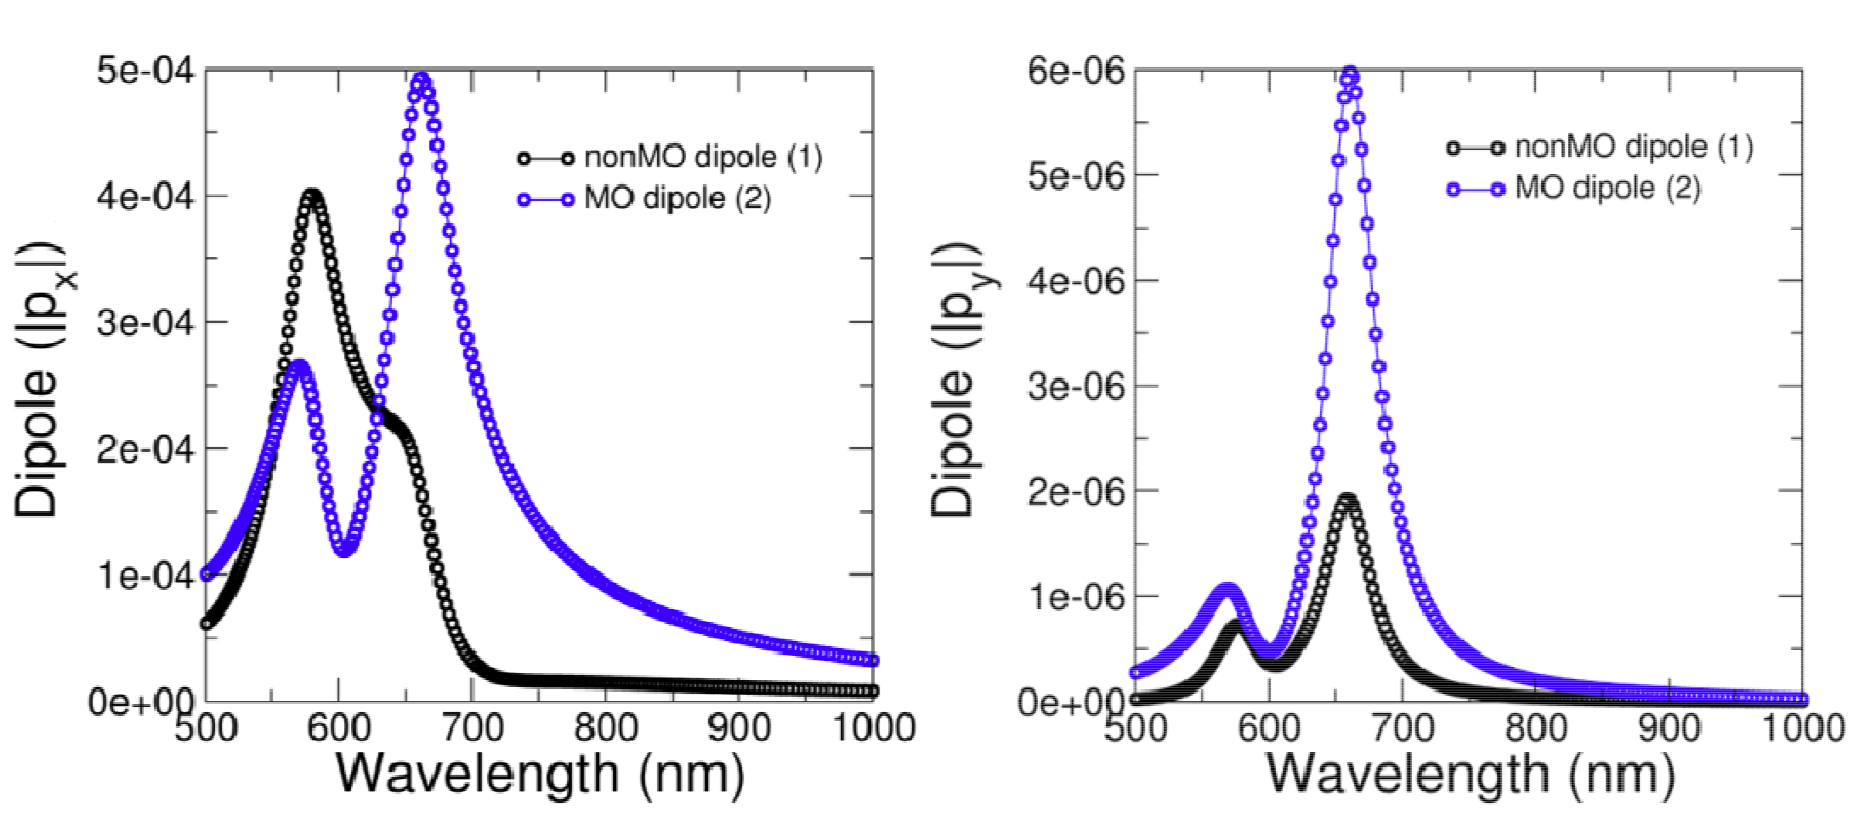
\includegraphics[width=12cm]{chapter_3/graphics/Fig_7.png} 
\caption{Wavelength dependence of the normalized dipole magnitudes along the $x-$ (left panel) and $y-$ (right panel) directions obtained using a point dipole model.\label{fig:dip_result}}
\end{figure}

In Fig. (\ref{fig:dip_result}) is shown the results obtained from Eq. (\ref{eq:chap3_polarizations_solution}) for intermediate interaction. Like in the mechanical case, the electric field is applied in the $x-$direction and only one of the dipoles is MO. Due to the electromagnetic coupling, both exhibit polarisation in the $y-$component.

The interaction between the electric dipoles gives rise to bright and dark modes (or more precisely, superradiant and subradiant modes), whose spectral position and character can be tuned by the thickness of the separating dielectric \cite{dmitriev2007gold, pakizeh2008structural, ekinci2008electric}. In the simple model presented here and schematically shown in Fig. (\ref{fig:scheme_springsdipoles})(b), left side, the bright mode corresponds to the configuration in which the electric dipoles are oriented parallel to each other (symmetric mode), while in the dark case the dipoles are oriented antiparallel (anti-symmetric mode). In both cases the electric dipoles are along x axis (parallel to the electric field of the incoming light). If one of the disks has ferromagnetic character, the application of a magnetic field along $z-$direction will induce a rotation of its associated dipole about this axis (Fig. (\ref{fig:scheme_springsdipoles})(b), right side). Extrapolating what it is obtained in the spring-mass case, the transverse oscillation induced in the uncharged mass will manifest here as an induced rotation of the dipole of the non-ferromagnetic metallic disk. The combined rotation of both dipoles will cause polarisation conversion effects. In this sense, magneto-optics is the appropriate tool to explore this new degree of freedom, since it provides a direct measurement of the magnetic field induced polarisation conversion.

\section{Optical and magneto-optical response of nanoresonators \label{sec:chap3_nanoresonators}} 

In order to confirm the previous results, we analyse structures that consist of a pure $\textnormal{Au}$ nanodisk separated by a $\textnormal{SiO}_{2}$ spacer from a $2nm\textnormal{Co}/4nm\textnormal{Au}$ multilayer nanodisk. The presence of $\textnormal{Au}$ in the bottom magnetoplasmonic disk reduces its optical losses as compared to a pure ferromagnetic metal disk \cite{armelles2013magnetoplasmonics}. The disks were fabricated using hole-mask colloidal lithography and evaporation (electron beam evaporation for $\textnormal{Co}$ and $\textnormal{SiO}_{2}$ layers and thermal evaporation for $\textnormal{Au}$ layers) \cite{banthi2012high, fredriksson2007hole}. In Fig. (\ref{fig:SEM_disk})(a) we show a sketch of the internal structure of each disk with the characteristic individual layer thickness. The $\textnormal{Au}/\textnormal{Co}$ multilayer disk exhibits perpendicular magnetic anisotropy, reducing the magnetic field required to achieve saturation in polar configuration, Fig. (\ref{fig:SEM_disk})(b). Fig. (\ref{fig:SEM_disk})(c) presents a cross section Scanning Electron Microscopy image of the same structure showing the truncated nanocone shape of the obtained nanoresonators, whose typical lower and upper disk diameters are $110-120nm$ and $70-90nm$ respectively. In this cross section image, both the metallic and dielectric components of the nanodisks are clearly distinguishable. Additionally, in Fig. (\ref{fig:SEM_disk})(d) a top view image of a representative structure, showing the homogeneous distribution of the disks over large areas, is presented.

\begin{figure}[h!]
\begin{centering}
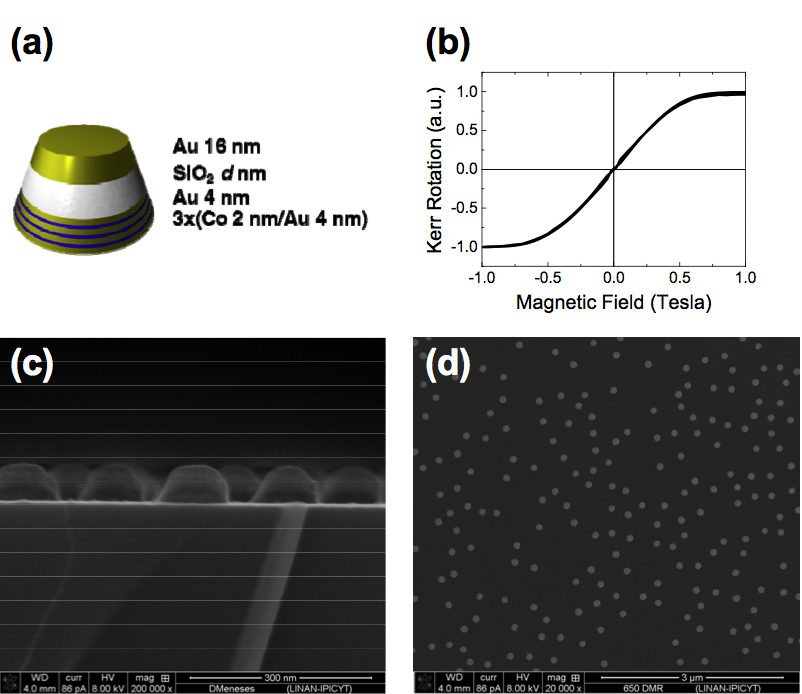
\includegraphics[width=10cm]{chapter_3/graphics/Fig_2.png} 
\par\end{centering}
\caption{(a) Schematic drawing of the nanoresonators composed of a purely plasmonic $\textnormal{Au}$ disk and a magnetoplasmonic $\textnormal{Au}/\textnormal{Co}$ superlattice disk separated by a dielectric spacer. (b) Polar Kerr loop of a characteristic sample. The presence of multiple $\textnormal{Co}/\textnormal{Au}$ interfaces reduces the value of the magnetic field needed to saturate the nanodisks in the direction perpendicular to the sample plane. (c), (d) Cross section and planar view SEM pictures, respectively, of a representative sample. The images show the homogeneous and random distribution of nanoresonators and their truncated conical shape and internal structure.\label{fig:SEM_disk}}
\end{figure}

In the left column of Fig. (\ref{fig:exp_extintion}) is shown the measured extinction spectra as a function of the $\textnormal{SiO}_{2}$ spacer thickness. As it can be seen, the spectral dependence of the extinction strongly varies as a function of the dielectric thickness, {\it{i.e.}}, with the inter-disk interaction. For the extreme case of thick $\textnormal{SiO}_{2}$ $\left(50 nm\right)$, both metallic disks interact weakly, and as a consequence two peaks corresponding to the individual disk resonances are observed. Thus, the high-energy peak can be identified with the resonance of the top metallic disk (smaller diameter) and the low energy one with that of the bottom one (larger diameter). As the $\textnormal{SiO}_{2}$ spacer gets thinner, the position and relative intensity of both resonances changes. In this situation, both modes become hybridised \cite{prodan2003hybridization, dmitriev2007gold} and we can no longer talk of individual modes but of complex modes of symmetric and anti-symmetric character. The symmetric mode, occurring at higher energies, strongly couples to the incident light and as a consequence has a larger extinction (bright or superradiant mode). On the other hand, the anti-symmetric mode, occurring at lower energies, couples weakly to the light, resulting in a lower extinction peak (dark or subradiant mode). Qualitatively, the symmetric mode is clearly observed for all the structures, while the anti-symmetric one gradually decreases in intensity, shifting to lower energies as the spacer becomes thinner, becoming practically unobservable for ${2}$ thickness below $15 nm$.\\

\begin{figure}[h!]
\begin{centering}
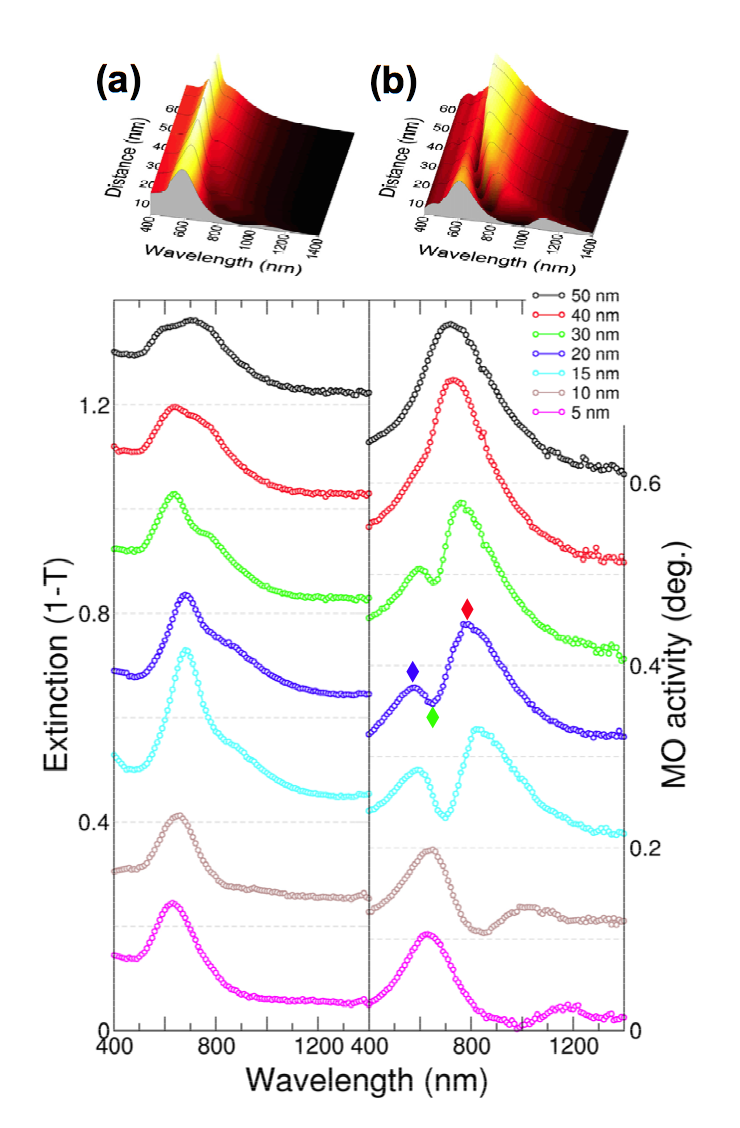
\includegraphics[width=8cm]{chapter_3/graphics/Fig_3.png} 
\par\end{centering}
\caption{(a) Extinction and (b) MO activity spectra of the nanoresonators as a function of $\textnormal{SiO}_{2}$ thickness. The different dashed horizontal lines indicate the zero value for each spectrum above the line. The 3D graphs on top of each panel show the results obtained from theoretical calculations of the same structures. The blue, green and red diamonds appearing in the experimental MO response for $20 nm$ $\textnormal{SiO}_{2}$ correspond to the spectral positions where the $E_{z}$ field distributions are calculated (see Fig. (\ref{fig:colormaps})).\label{fig:exp_extintion}}
\end{figure}

The right hand column of Fig. (\ref{fig:exp_extintion}) shows the spectral dependence of the MO activity of the same nanostructures, corresponding to the modulus of the complex Polar Kerr rotation, $\Phi$ (where $\Phi = \theta + i\phi$, being $\theta$ and $\phi$ the Polar Kerr rotation and ellipticity respectively, as presented in Sec. (\ref{sec:chap2_dielectric_tensor})), measured at normal incidence and magnetic saturation. Unlike simple fully metallic $\textnormal{Au}/\textnormal{Co}/\textnormal{Au}$ nanodisks where MO activity and extinction spectra are directly related \cite{gonzalez2008plasmonic}, the spectra of our nanodisk dimers exhibit a strong dependence on the spacer thickness but with distinctive differences with respect to the extinction spectra. For example, for thick spacer layers only one peak is observed, contrary to the double peaked spectral dependence of the extinction. This peak corresponds to the MO activity of the bottom disk, which actually is the only one with a ferromagnetic constituent. The upper disk, made up of pure $\textnormal{Au}$, does not contribute to the MO activity of the structure. However, as the $\textnormal{SiO}_{2}$ becomes thinner and the electromagnetic (EM) interaction between both metallic disks increases, a new peak appears at higher energy, whose position hardly depends on the spacer thickness. On the other hand, the low energy MO peak gradually red shifts and loses intensity as the spacer thickness is reduced. Additionally, and contrary to what was observed in the extinction measurements, this low-energy peak is observed all the way down to the thinnest dielectric spacer in the MO case. Special mention deserves the specific MO peak shapes for intermediate spacer thickness (between $15$ and $30 nm$), where the two MO peaks are energetically close. In this regime the MO spectra are clearly not the result of the convolution of two peaks that would originate from independent modes, but rather exhibit a typical Fano resonance shape, which on the other hand is absent in the extinction spectra.\\
To further link the experimental results with the dipole model, we have performed rigorous simulations for both the extinction and MO response, based on scattering matrix techniques \cite{garcia2005light, caballero2012generalized} and FDTD \cite{lumericalcite} as well as FEM \cite{comsolcite} codes. The three methods provide equivalent results. The evolution of the spectra as a function of the $\textnormal{SiO}_{2}$ thickness is depicted as 3D graphs on top of the corresponding columns in Fig. (\ref{fig:exp_extintion}), exhibiting a very good agreement with the experimental results, both regarding the intensity, spectral shape, and peak position evolution. In addition to the mentioned extinction and MO activity, the performed simulations allow also obtaining the EM field distribution in regions around the nanodisks. As an example we present in Fig. (\ref{fig:colormaps}) the near field distribution of the $z-$component of the electric field, for the sample with $20nm$ $\textnormal{SiO}_{2}$ spacer, in two planes at $10 nm$ above the top and below the bottom disks respectively, both in the absence of an external magnetic field and as the difference for magnetic saturations along opposite directions. These distributions have been calculated for the three wavelengths corresponding to the two maxima and the minimum of the MO activity (labelled with red, green and blue diamonds in Fig. (\ref{fig:exp_extintion})).\\
The $E_{z}$ component without external magnetic field (extinction measurements situation) is presented in the left panel of Fig. (\ref{fig:colormaps}). There, for the low energy position (red framed) the EM distribution for each metallic disk resembles that of a point dipole oscillating along the $x-$direction, with similar $E_{z}$ intensity for both upper and lower disk, and with the individual dipoles (represented by the black arrows in Fig. (\ref{fig:colormaps})) oriented antiparallel (note that the $E_{z}$ field of a dipole changes sign when it is seen from above or from below). This situation therefore corresponds to the aforementioned anti-symmetric configuration. On the other hand, for the high energy position (blue framed) the EM distribution for each metallic disk corresponds also to a dipole-like distribution along the $x-$direction but now the individual dipoles corresponding to the disks are oriented parallel to each other (symmetric mode). As it can be seen, the intensity of the $E_z$ component for both disks is, again, similar, but larger than that for the low energy case. This is consistent with the higher extinction value obtained for the symmetric mode respect to the anti-symmetric one. Finally, at the intermediate energy (green framed), the distribution is still dipolar-like and would correspond to a symmetric-like mode, but the intensity distribution is not equally distributed, with a larger value of the $E_z$ component in the upper disk than for the lower one.

\begin{figure}[h!]
\begin{centering}
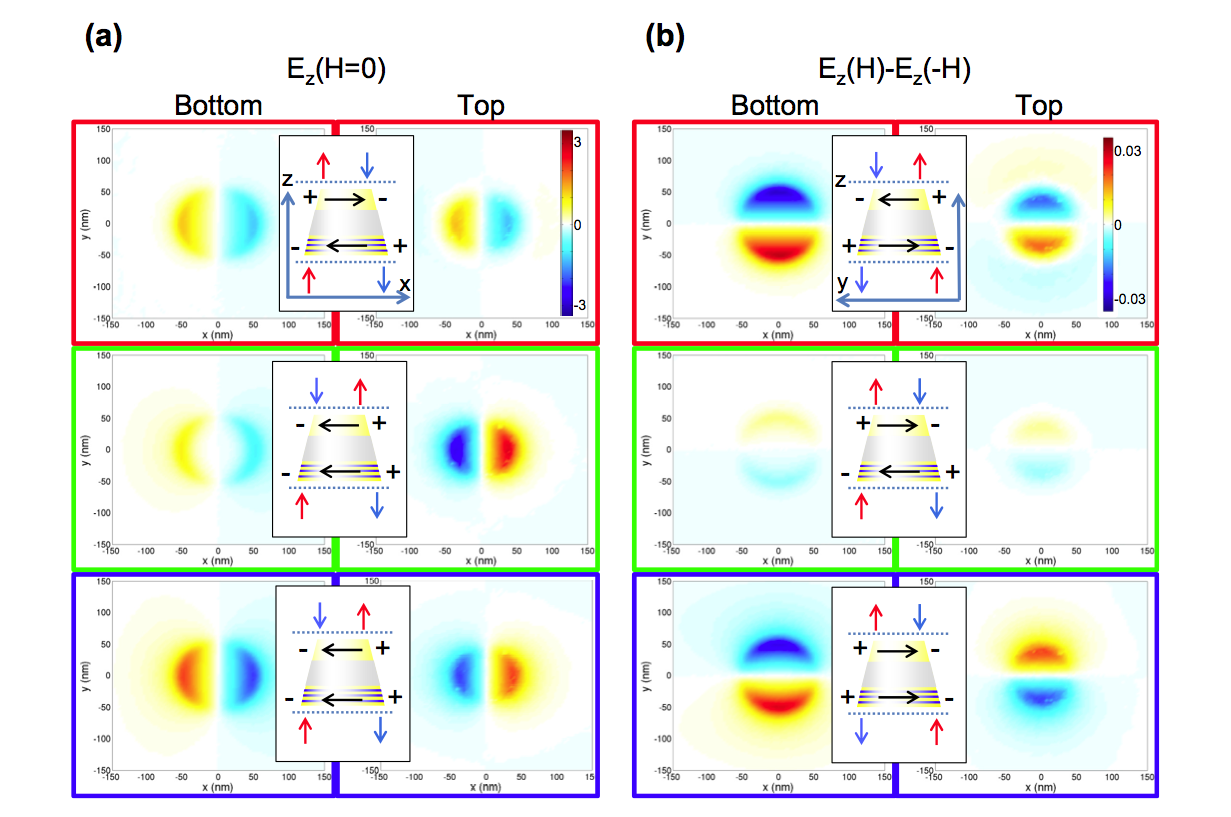
\includegraphics[width=12cm]{chapter_3/graphics/Fig_4.png} 
\par\end{centering}
\caption{(a) Calculated near field intensity of the $E_z$ component for a nanoresonator with $20$ nm $\textnormal{SiO}_2$ spacer in two planes above the top disk and below the bottom one, with the incident field polarised along the $x$ direction and in the absence of an external magnetic field. This distribution reflects the excitation of two dipoles along the $x$ direction. The insets indicate the corresponding charges and dipole orientations (indicated by the black arrows) according to the $E_z$ distribution for the different cases. The red (blue) arrows in the insets represent the positive (negative) values of the $E_z$ field component. (b) Difference of the $E_z$ components for magnetic saturation along opposite directions in the same planes and for the same structure. This difference accounts for the effect of the applied magnetic field: The appearance of a dipole along the $y-$direction for both the magnetoplasmonic (intrinsic dipole) and the plasmonic (induced dipole) disks. In both cases, the components for three different wavelengths labelled as diamonds in Fig. (\ref{fig:exp_extintion}) are shown.\label{fig:colormaps}}
\end{figure}

Next, in the right panel of Fig. (\ref{fig:colormaps}) we show the difference between $E_z$ components at magnetic saturation along opposite directions, $E_{z}(H)-E_{z}(-H)$ (MO measurements situation) which reflects the magnetic field effect on the field distributions of the system eliminating the purely optical contribution. For the three energies, a dipolar-like distribution is still observed, but the resulting balance between magnetic saturation along opposite directions is an $E_{z}$ component corresponding to a point dipole oscillating along the $y-$direction. In other words, the effect of the magnetic field is to induce a "dipole" along the $y-$direction that is two orders of magnitude smaller in intensity than the dipole generated along the $x-$direction.\\
On the other hand, regarding the symmetry character of the resulting modes, it is maintained for high and low energies with respect to the case of no magnetic field applied: anti-symmetric and symmetric for low and high energy respectively. Regarding the intensities of the $E_{z}$ fields, it is similar for top and bottom disks and for both energies. The induction by the magnetic field of a dipole along $y-$direction is pretty intuitive for the bottom disk, since it is simply due to the presence of ferromagnetic material in it. What is in principle not as intuitive is the presence of the same component in the upper disk, since it has no ferromagnetic nature. This $y-$component in the upper disk is induced by the "dipole" of the bottom disk, reaching a sizeable magnitude. More interestingly, the situation for the intermediate energy, corresponding to the minimum of the MO activity, is quite different. In this case both lower and upper disks, regardless the presence of a ferromagnetic component in its interior, exhibit almost zero MO-induced "dipoles".

\section{Discussion\label{sec:chap3_discussion}}

From the observation of the resulting $E_{z}$ components, one can conclude that the application of a magnetic field has three main effects: first, it generates a "dipolar" component along the $y-$direction not present without magnetic field; second, mediated by the interaction between the disks, the bottom disk, which has a ferromagnetic component, induces a "dipole" along the $y-$direction in the upper disk, in other words it generates a MO activity in a disk which has no ferromagnetic nature; third, there is a spectral region were both "dipoles" vanish almost completely, and therefore, the MO activity is strongly reduced.\\
To understand the physical origin of this phenomenology, let us consider the field distributions obtained for the intermediate energy region shown in the left panel of Fig. (\ref{fig:colormaps}). In that region, the intensity of the field at the bottom disk clearly decreases with respect to the other two energies considered. This suggests that the electric field induced by the upper disk destructively interferes with the incoming electric field. This can be understood from the simple model based on two interacting point dipoles. From the solution of the dipole model, Eq. (\ref{eq:chap3_polarizations_solution}), is identified a common term $\left[e^{i\delta}+k^2{\cal{G}}\alpha_{1}\right]$ for both $x-$ and $y-$components of the dipole with MO activity ($\bold{p}_2$) and the $y-$component of the dipole with no MO activity ($\bold{p}_1$). This term is related to the total electric field along the $x-$direction at the MO active dipole, and results from the addition of the incident field and the field generated at this point by the dipole with no MO activity. If this term vanishes the three components die out, and therefore the MO activity is suppressed. On the other hand, as the $x-$component of the dipole with no MO activity does not depend on this term, it is not cancelled being the only one that contributes to the optical response of the whole system. From the point of view of the mechanical model this situation corresponds to the transition region between the in-phase and out-of-phase oscillations of the masses: the charged mass decreases its oscillation and therefore the Lorentz force, proportional to the velocity, is strongly attenuated. As a consequence, the movement of this mass along the $y-$direction and the induced movement of the uncharged mass are also reduced.\\
This phenomenon can be viewed as the MO counterpart of the electromagnetic induced transparency. For a specific spectral region, the EM interaction between the two disks gives rise to a situation where the total EM field at the MO active element is minimised, therefore strongly reducing the MO activity of the whole system, (see Eq. (\ref{eq:chap3_polarizations_solution})). This is observed in Fig. (\ref{fig:chap3_MO_activity})(a), where we present the experimental MO activities for two different situations corresponding to very weak interaction (the $50 nm$ $\textnormal{SiO}_2$ structure) and a situation where the two disks clearly interact (the $20 nm$ $\textnormal{SiO}_2$ structure). For the very weak interacting system only a broad peak is observed, corresponding to the MO activity of the magnetoplasmonic disk. However, for the system where the two metallic disks interact, a narrow dip with a clear Fano-like shape is obtained. The difference between both spectra is also shown (inset), presenting a narrow peak.\\
\begin{figure}[h!]
\begin{centering}
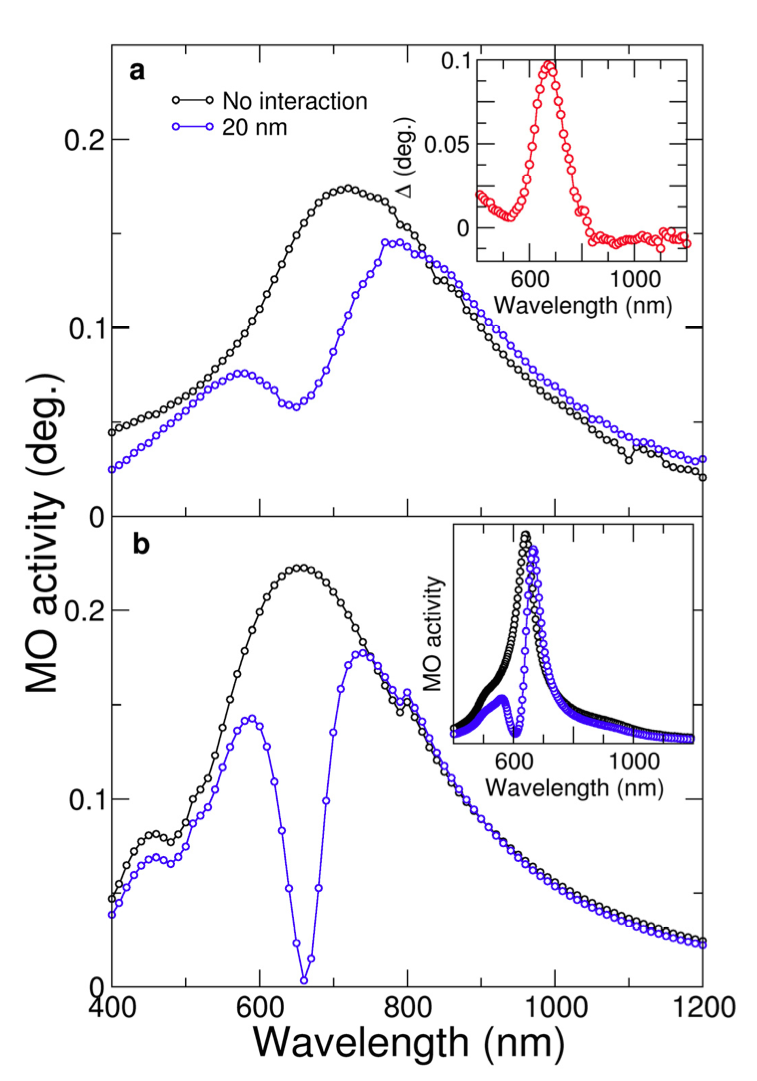
\includegraphics[width=8cm]{chapter_3/graphics/Fig_5.png} 
\par\end{centering}
\caption{Fano resonance in the magneto-optical activity. (a) Experimental spectra of the MO activity for the structures with $20 nm$ and $50 nm$ $\textnormal{SiO}_2$ spacer, corresponding to interacting and non interacting situations, respectively. For the interacting situation a clear Fano resonance shape is observed. The inset shows the difference between the two spectra, resulting in a narrow peak.\\
(b) Theoretical MO activity spectra obtained for a structure with $20nm$ $\textnormal{SiO}_2$ spacer and for the same structure but without the upper metallic disk. The inset shows the MO spectra obtained using the simple point dipole model.\label{fig:chap3_MO_activity}}
\end{figure}
Fano resonances are observed whenever a broad and a narrow state interfere destructively, giving rise to a sharp spectral feature. In our specific case, the broad state corresponds to the EM field at the MO disk in the absence of interaction, whereas the narrow one is due to the electromagnetic field induced by the non-MO disk at the MO disk. Due to its intrinsic interaction origin, this Fano shape strongly depends on the $\textnormal{SiO}_2$ spacer thickness. As it can be seen in Fig. (\ref{fig:exp_extintion}), for thick enough $\textnormal{SiO}_2$ spacers, the MO activity is simply that of an individual disk (the bottom disk) and, as the spacer thickness is gradually reduced, the interaction between the disks becomes more relevant and, especially for intermediate spacer thickness, the Fano-like shape is clear. This interaction dependence appears explicitly in the common term of Eq. (\ref{eq:chap3_polarizations_solution}) as the field propagator ${\cal{G}}$ depends on the distance between the two dipoles. In Fig. (\ref{fig:chap3_MO_activity})(b) we also present the calculated MO activity using a transfer matrix formalism or a simple dipolar model (inset) for two cases corresponding to a structure without the upper disk (no interaction) and a structure with both disks separated by a $20 nm$ thick $\textnormal{SiO}_2$ layer. As it can be observed the calculated results follow the same trends as the experimental ones.

\section{Conclusion \label{sec:chap3_conclusions}}
In conclusion, MO activity in non-MO elements can be induced via electromagnetic interaction with MO active elements. This effect has been shown in magnetoplasmonic resonators consisting of a $\textnormal{Au}$ plasmonic disk separated by a $\textnormal{SiO}_{2}$ layer from a MO active magnetoplasmonic $\left(\textnormal{Au}/\textnormal{Co}\right)$ disk. When a magnetic field is applied perpendicular to the disks, it produces an electric dipole along the perpendicular direction of the electric field of the incoming light in the MO active disk. This electric dipole induces a MO activity in the non- magnetic $\textnormal{Au}$ disk. Additionally, we have shown the existence of an electromagnetically induced magneto-optical transparency in these systems. This is due to the interference at the MO disk between the incidence electromagnetic field and that generated by the non-MO one, leading to a Fano-like spectral dependence of the MO activity and to a strong reduction of the MO activity. This may find applications in sensing architectures based on MO-Fano resonances. Optical Fano resonances have already demonstrated their potential applicability \cite{yanik2011seeing, wu2012fano, offermans2011universal}. Additionally, plasmon excitation enhancement of the MO activity has also shown improvement of the performance of standard plasmonic sensors \cite{sepulveda2006highly, bonanni2011designer}. Combining both effects may allow the generation of novel sensing platforms based on MO-Fano resonances. Since the observed phenomenon is driven by the resonance of the upper disk, modifications of the dielectric environment may strongly affect it and, as a consequence, the overall observed Fano resonance characteristics.

